\newcommand{\maxn}{100}
\newcommand{\maxk}{10}
\newcommand{\maxq}{2500}

\begin{frame}
    \frametitle{\problemtitle}

    \begin{columns}
        \begin{column}[T]{.70\textwidth}
            \begin{itemize}
                \item Interactively play \emph{Battleships} with an $n \times n$ grid ($5 \leq n \leq \maxn$).
                \item Sink $1 \leq k \leq \maxk$ aircraft carriers (size $1 \times 5$) in at most $\maxq$ shots.
                \item The interactor is adaptive:
                    the placement of the ships may be determined during the interaction,
                    and may depend on where you decide to shoot.
                    It is guaranteed that the final placement of the ships
                    will be consistent with the responses to all your shots.
            \end{itemize}

            \vspace{1em}

            \centering
            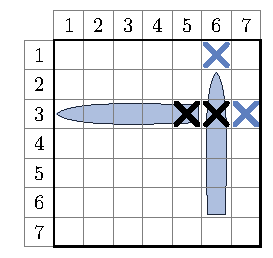
\includegraphics[width=0.3\textwidth]{sample}

            \small
            Illustration of Sample Interaction 1 after the first four shots were fired.
        \end{column}

        \illustration{0.25}{battleships.jpg}{
            The original \emph{Battleships} game, \\
            before the upgrade to a $\maxn \times \maxn$ grid. \\
            CC BY-NC 3.0 by Pavel Ševela \\
            on \href{https://commons.wikimedia.org/wiki/File:Hra_n\%C3\%A1mo\%C5\%99n\%C3\%AD_bitva_(1).jpg}{Wikimedia Commons}
        }
    \end{columns}
\end{frame}
